\section{Proposed Approach} \label{sec:approach}
 
\subsection{Dataset and Preprocessing} \label{sec:dataset}

The dataset we will be utilizing is the UTKFace dataset,
which consists of $23,708$ aligned and cropped facial images, 
annotated with age, gender, and ethnicity labels.
This dataset was created with the intention of covering
a wide range of variations, including pose, facial expression,
illumination, occlusion, resolution, and more.
In our analysis, we will specifically concentrate
on the first two attributes within the dataset: age and gender. 

In our analysis, we will exclusively consider $70\%$
of the dataset for our training set, with the remaining
$30\%$ designated for testing purposes.
This division allows us to train our models on a substantial
portion of the data while maintaining a separate,
untouched set for rigorous evaluation.

The training set exhibits an age distribution depicted
in the histogram
shown in Fig.~\ref{1age}, along with a balanced gender distribution,
as illustrated in Fig.~\ref{2gender1}.

\begin{figure}[htbp]
    \centerline{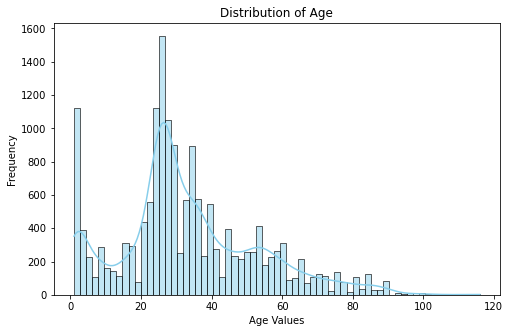
\includegraphics[width=.5\textwidth]{images/dataset/age.png}}
    \caption{Histogram of age distribution in the training set}
    \label{1age}
\end{figure}

\begin{figure}[htbp]
    \centerline{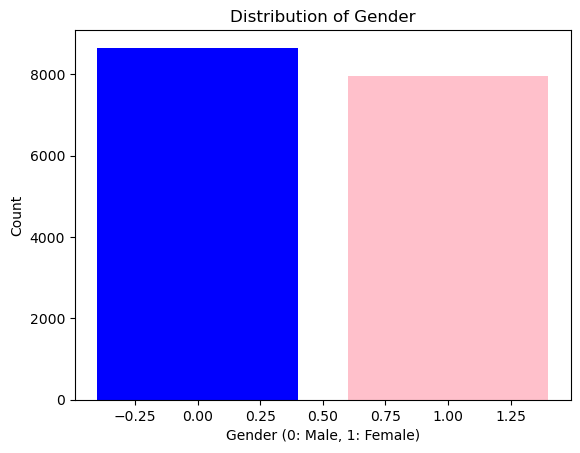
\includegraphics[width=.4\textwidth]{images/dataset/gender1.png}}
    \caption{Histogram of gender distribution in the training set}
    \label{2gender1}
\end{figure}

We further split the training set into a $70\%$ training set and a $30\%$
validation set. The validation set plays a critical role in refining
and making our model more robust, preventing overfitting through techniques
such as early stopping.

Despite this subdivision, we have taken measures to maintain the
balance in the dataset: the accompanying histogram in  illustrates that,
concerning gender, the distribution remains similar in both datasets.

\begin{figure}[htbp]
    \centerline{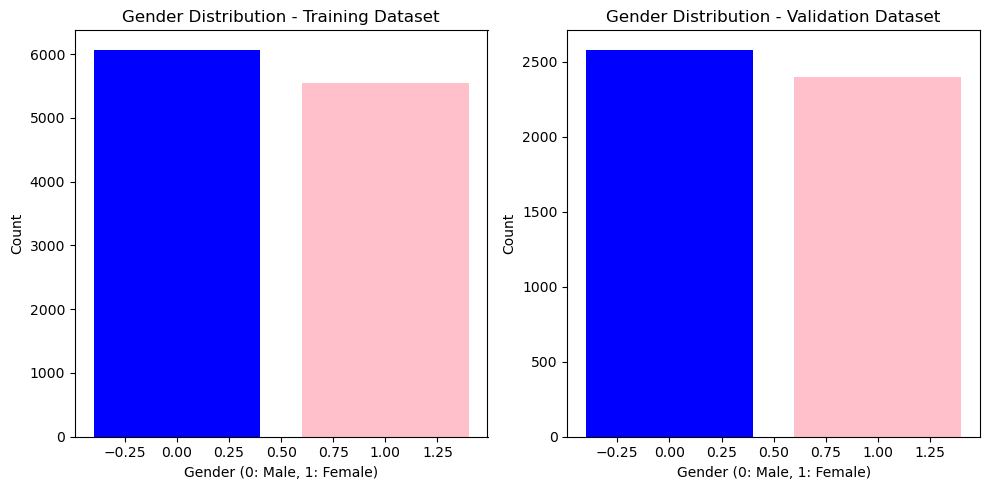
\includegraphics[width=.5\textwidth]{images/dataset/gender2.png}}
    \caption{Histogram of gender distribution in the new training
    set and the validation set}
    \label{3gender2}
\end{figure}

As for age, a continuous value that poses challenges for balance
assessment, we will employ the non-parametric Kolmogorov-Smirnov test
to scrutinize the absence of statistically significant differences in
the distributions of its values between the two datasets
(its null hypothesys) \cite{app1}.
The outcome of the aforementioned test yields a $p$-value of approximately
$0.38$, this value is reasonably high,
leading us to consider it sufficient evidence to accept the null hypothesis.
Thus, we conclude that the two distributions of age in the two
datasets do not exhibit statistically significant differences.

The concluding step in our dataset preprocessing involves the application
of data augmentation techniques. Specifically, we expand the dataset
by incorporating horizontally mirrored images and introducing random
rotations of up to 10 degrees. Additionally, we employ random adjustments
to the brightness, contrast, saturation, and hue of the images.
This augmentation strategy has been employed based on empirical
evidence suggesting that enlarging the dataset enhances the model's
performance. By introducing these variations in orientation and color,
we aim to expose the model to a more diverse set of examples,
ultimately improving its ability to generalize and make accurate
predictions on unseen data.

\subsection{Model Architecture} \label{sec:model}

As previously mentioned, in this project, we will compare two
CNN architectures, one comprising a single multi-task
network and another consisting of two single-task networks.
The overarching goal is common between them.

Let's delve into the details of the first architecture.

\subsubsection{Multi-task Network} \label{sec:multi}

